
\chapter{Collaboratively running experiments}
\begin{figure}[h] 
  \centering
  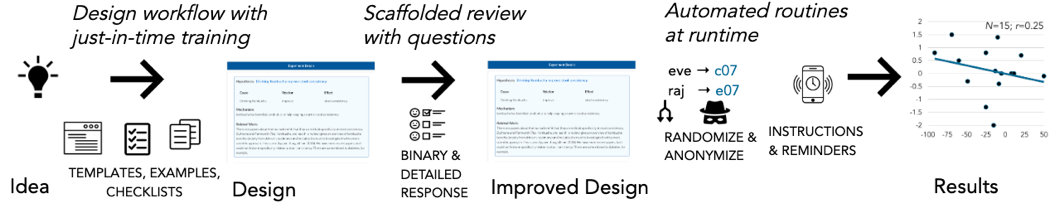
\includegraphics[width=1.0\textwidth]{figures/galileo/galileo-1}
  \caption[]
{Galileo enables anyone to design and run experiments to test their intuitions. Experiment creators can invite anyone to review and participate in the experiment. Participants from around the world join experiments, follow instructions, and provide data in response to automated data collection reminders.\index{galileo-1}}
  \label{fig:galileo-1}
\end{figure}

Scientific experimentation features technical requirements and contextual choices that are inscrutable for a lay individ-ual yet necessary for success~\cite{Martin2007}. While professional scientists and commercial ventures run experiments every day, with notable exceptions~\cite{Cooper2010, Lewis2016}, empirical papers from non-professionals are vanishingly rare. This biases the questions asked, studies run, and knowledge created~\cite{crawford2017politics,Henrich2010a}. People have questions about their health, but lack the expertise and resources to scientifically investigate them. Broadening the pool of experimenters could help people investigate their curiosities, develop solutions to improve health and performance, and assist institutional researchers.

The main contribution of this paper is demonstrating that online volunteers can collaboratively perform scientific experimentation. It does so in two main ways: 1) proce-dural support for acquiring domain expertise using three techniques: experimental design workflow that provides just-in-time training, review with scaffolded questions, and automated routines for data collection; and 2) the Galileo social computing system that instantiates procedural support for citizen experimentation (Figure~\ref{fig:galileo-1}). 

Three empirical investigations tested Galileo’s approach. First, a controlled between-subjects experiment with 72 participants found that procedural support yielded signifi-cantly higher-quality experiment designs than lecture videos. Second, a deployment across 16 countries found that people generated structurally-sound experiments on personally meaningful topics. Third, in a field deployment, online users from three communities—kombucha, Open Humans, and beer—across 8 countries demonstrated that people designed, iterated on, and ran week-long experiments.

\section{Related Work}
\subsection{Citizen Scientists: From Collectors to Experimenters}
Citizen science efforts span counting bird species, identify-ing galaxies, editing protein structures, and creating novel hypotheses [15,56,69]. One reason for citizen science’s success is that different people provide different expertise that can vet claims and fix mistakes [35]. A humbling example of the power of fresh eyes: volunteer citizen scientists identified an entirely new class of galaxies (“green pea” galaxies) from Galaxy zoo images; experts had dismissed these images as apparatus error [7]. This volun-teer-led discovery demonstrates the need for fostering independent perspectives while simultaneously cultivating sufficient knowledge for meaningful domain contributions. 

Efforts to expand participation in scientific research are bearing fruit: Lab in the Wild recruits anyone with an internet connection for behavioral studies [58]; All of Us aims to recruit one million Americans from all strata of society (allofus.nih.gov). Distributed data contributions from people around the world—browsing online [17], using activity trackers, and joining scientific projects—have enabled valuable insights on topics including obesity [2], aesthetic preferences [59], sleep [25], and the human microbiome [52]. Our work draws on the idea of people using their complementary insights and cognitive surplus towards expert-led scientific work [5].

A number of health and behavioral research projects enlist citizens as helpers (e.g., HabitLab [43]). It remains rare for citizens to design experiments. CivilServant enables online communities’ moderators to test policy ideas; moderators share these ideas with researchers who transform them to study designs [51]. Through the PatientsLikeMe website (patientslikeme.com), citizens and scientists created a study investigating whether consuming lithium alleviated ALS symptoms [64]. While an initial scientific study had provided positive benefits, both this citizen science study and a subsequent university study did not find benefits. Closest to our research, Tummy Trials asked participants to generate health questions, introducing a protocol for self-experimentation combining ideation and self-tracking [36].

This paper provides a general workflow for anyone to transform their intuition to an experimental design; our work focuses on controlled experiments as opposed to self-tracking or informal iteration.

\subsection{Supporting novice inquiry}
Lived experience, a tight feedback loop, and strong personal motivation can yield different and sometimes better ideas than experts [33]. Prior work has explored collaborative hypothesis generation and testing on pre-existing data sets [48,67]. Galileo offers a complementary contribution: enabling citizens to generate data on topics of personal interest.

One way to make complex tasks manageable is to divide them into distinct phases. Touchstone demonstrates the power of a semi-automated workflow integrating experi-ment design, testing, and analysis [49]. Crowdsourcing has similarly innovated by creating distinct phases: break larger tasks into microtasks; algorithms specify the division, dependency, and agglomeration activities while workers perform small tasks supported by task-specific guidelines [45]. From these systems, our work draws the idea of dividing experimentation into multiple tasks—some self-sourced, others crowd-sourced; and introduce just-in-time domain expertise to perform these tasks. 

Carefully-constructed interfaces can aid novices with task-specific expertise to solve problems that only experts previously could. Foldit introduced 3D game for specifying low-energy protein structures via direct manipulation [15]. Making a challenge visually salient is an effective way to on-board novices. This paper explores scaffolds that are more structural than visual.

Providing just-in-time supports, step-by-step instruction, and showing helpful supportive information are core ideas in instructional design [39]. Crowdsourcing systems leverage interactive guidance for specific tasks. For exam-ple, CrowdLayout and Cicero provide guidelines and static rules that workers use these to reason about their choices and improve network layouts [11,62]. Others like CrowdSCIM and Crowdclass scaffold pre-task interventions [46,63]. Galileo introduces support during the task itself for those with little-to-no mental model of the knowledge domain. Like the Shepherd review-writing system [20], Galileo provides just-in-time support. There are two key differences: 1) Galileo scaffolds the entire creation process, not just the post-draft feedback stage, and 2) Galileo does not draw on expert time – the knowledge is implemented in the software itself. 

\section{The Galileo Experimentation platform}
Galileo introduces a system for end users to design experi-ments, get them reviewed, and run them with interested participants. It provides procedural support for these steps, an online collaboration platform, and automated data collection and reminders (Figure 1).

Despite a predetermined goal and a formalized process, experimentation requires making contextually-appropriate decisions [50]. Good experiment design is inherently user centered; designers need awareness of others’ interpretation of their ideas and asks. Providing feedback on experiment designs requires knowing the success criteria and how to help improve. Finally, successfully running an experiment requires managing multiple processes such as random assignment, anonymizing participant details, and sending instructions and reminders for data collection.

\subsection{Design-Review-Run: From Intuitions to Investigations}
Galileo requires three roles for each experiment: designer, reviewer, and participant. Galileo offers procedural support for each: 1) a design workflow provides just-in-time training, 2) review with scaffolded questions, and 3) automated routines for runtime activities like data collec-tion. Users form and refine with the help of contextual support and learning resources from the system. 

\subsubsection{Design an Experiment from an Intuition}
People have many, often poorly-framed, hypotheses. Galileo’s design workflow helps people harvest and sharpen them (Figure 2). Examples illustrate possible choices and how they relate; templates provide structure; and embedded videos explicate technical issues. Such procedural support can improve on-task performance [56]. A final self-review step provides an overview of the experiment. To keep the platform safe, the primary author receives daily updates of platform activity. The design workflow does not mandate double-blindness or the use of placebo; designers can choose to specify these details.

\begin{figure}[h] 
  \centering
  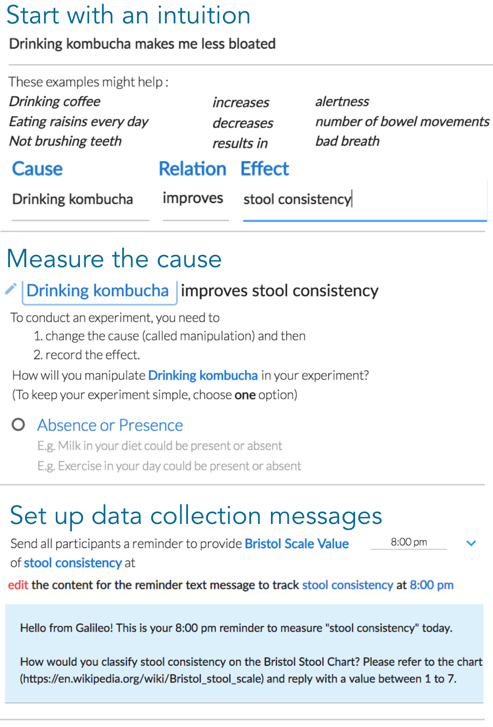
\includegraphics[width=0.5\textwidth]{figures/galileo/galileo-2-design}
  \caption[]
{Galileo’s design module helps people transform intuitions into experiment designs. It walks people through 1) convert-ing an intuition to a hypothesis, 2,3) providing ways to manipulate/measure cause and effect, 4-5) specifying control and experimental conditions, and (not shown) providing inclusion/exclusion criteria..\index{galileo-2}}
  \label{fig:galileo-2}
\end{figure}

\subsubsection{Review the Design via Feedback from Others}
Galileo experiments require at least two reviews before they can be run. The designer invites the reviewers, who might be online community members, a teacher, or anyone else who can provide useful feedback. Upon receiving reviews, the designer edits the experiment to address any issues. For research purposes, Galileo logs version changes. Reviewers provide both binary assessment and written responses to specific questions (Figure 3). These questions cover structure (e.g., accounting for confounds), pragmatics (e.g., measuring the real-world cause/effect), and participant experience (e.g., data reminder time). Reviewers are ineligible to be participants in the same experiment. Similarly, creators may not review their own experiment. 

\begin{figure}[h] 
  \centering
  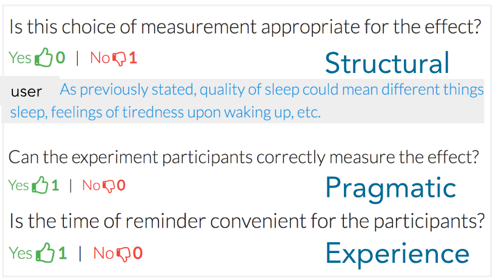
\includegraphics[width=0.5\textwidth]{figures/galileo/galileo-2-review}
  \caption[]
{Reviewers walk through an experiment providing binary rubric assessments. A No response prompts reviewers to provide concerns and suggestions.\index{galileo-2-review}}
  \label{fig:galileo-2-review}
\end{figure}

\subsubsection{Run an Experiment using Procedural Support}
To launch an experiment, its designer shares a unique URL with potential participants. Galileo automatically manages four activities to reduce bias and workload: 
1 Randomized placement of people into conditions [50].
2 Maintain a per-experiment participant map ([usernames]$\rightarrow$ [exp$\textunderscore$id]) for anonymity
3 Collect and clean data (sending data collection messages and reminders at time-zone appropriate times, parsing the responses, updating participant and experimenter views). 
4 Prompt experimenters to perform tasks when conditions are met (e.g., setting the start date when enough participants have joined or reminding participants with missing data). 

Participation comprises following instructions (e.g., drink kombucha) and providing self-report responses to platform queries (Figure 4). The current implementation supports email, SMS, and WhatsApp. Self-reports provide the primary data collection mechanism. Participants can optionally answer follow-up questions that capture contex-tual insights. Galileo logs responses to a MongoDB database. Galileo presents participant data to experimenters using participant ID rather than real name or username. When the experiment ends, participants receive a summary of results. Participants can anonymously discuss the experiment at the end, so the experimenter can learn from their feedback. 

\begin{figure}[h] 
  \centering
  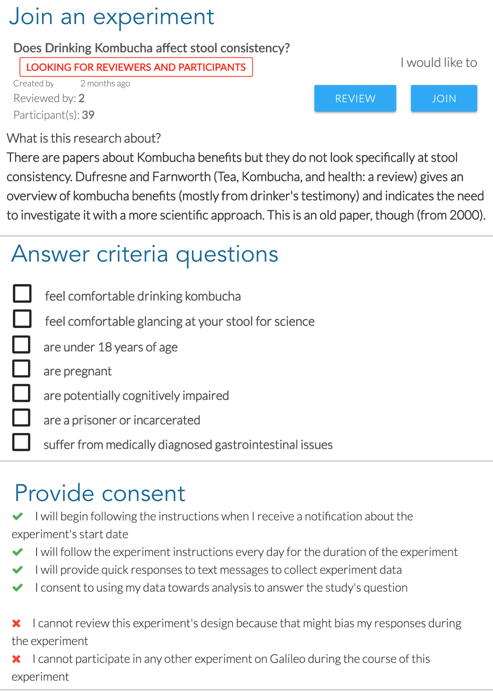
\includegraphics[width=0.5\textwidth]{figures/galileo/galileo-2-run}
  \caption[]
{1) Participants can view a list of experiments. When they elect to join one, they 2) answer inclusion/exclusion criteria, 3) consent to following the provided steps, and 4) receive instructions. Participants receive daily, condition-specific requests, and respond with data and/or clarifying questions. \index{galileo-2-run}}
  \label{fig:galileo-2-run}
\end{figure}

The experimenter’s dashboard lists tasks: answer clarifying questions, remind/thank participants, or look at trends in data (Figure 5). Experiments have a minimum participation count; there’s no upper limit to the number of participants. People who sign up after a cohort begins are added to a waitlist.
The Galileo web application uses the Meteor (meteor.com) framework for synchronization, Jade for the front end (jade-lang.com), Materialize for styling (materializecss.com), and Twilio as the text message gateway (twilio.com). Galileo can be used at <URL>; its open source is at <URL>. 

\begin{figure}[h] 
  \centering
  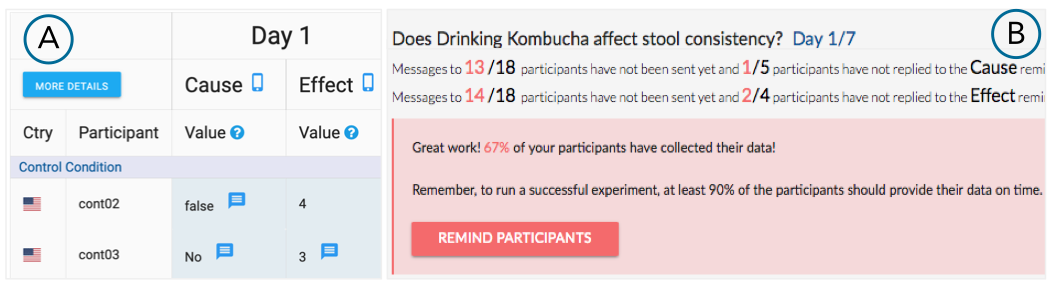
\includegraphics[width=0.5\textwidth]{figures/galileo/galileo-2-run-1}
  \caption[]
{Galileo takes care of many experimenter responsibilities such as random placement of people, sending instructions and reminders, and cleaning and displaying data in both participant and experimenter dashboard. The dashboard enables experi-menters to A) remind those with missing data; and B) see participants’ data; and clarify questions raised by participants. . \index{galileo-2-run-1}}
  \label{fig:galileo-2-run-1}
\end{figure}
 

\subsubsection{Designing the platform}
More than 80 people have designed and run experiments. The system design evolved over a year of weekly in-person user-centered studies with lead users from different commu-nities including kombucha and self-tracking enthusiasts. The pilot study gathered feedback on the usefulness of the interface items and resources. Students in an undergraduate Psychology class (Introduction to Research Methods) also used Galileo in a 90-minute classroom deployment to rapidly design and review each others’ experiments and receive feedback. We provide three examples of how pilot studies informed Galileo’s design:

1 Embedded written training over videos: Early versions provided short, online lecture videos as the learning materials. Most users did not watch them end-to-end to extract the step-relevant insight(s). In response, each step’s content now offers written examples, which are easier to skim and refer back to. 

2 Supporting actionable feedback: For the review interface, early versions only requested binary Yes/No responses similar to popular crowdsourcing platforms; both experi-ment designer and reviewers found this to be unsatisfactory. Galileo now provides a prompt for actionable feedback whenever the reviewer selects “No” to any question. 

3 Ease of glancing at participants’ data: Pilot users ran six trial experiments. The idea of a run-time dashboard (Figure 5A) came from observing experimenter’s difficulty tracking participants’ data and sending reminders to those who hadn’t added their data. Participants struggled with making suitable preparations for a week of experimentation (e.g. buying sufficient kombucha). The system now prompts experimenters to explicitly add preparation instructions that are sent to participants 2 days before the experiment begins. 

Integrating Procedural Support in the Design Workflow
Simple examples of procedural learning are activities like tying your shoes, roasting a chicken, or replacing a door handle. Recipes and instructions convey procedures in written form; demonstrations and hands-on learning make it more interactive. Creative tasks differ from rote procedures in that they require people to generate some artifact them-selves.

\subsubsection{Embedding Just-in-Time Support}
Complex activities overwhelm learners’ working memory because of their many interrelated pieces [23]. Recalling work from previous steps and frequent context-switching are especially taxing [27]. Experts mitigate memory demands by integrating multiple elements into conceptual chunks [10]. A well-chunked interface can still require knowledge that novices lack. Galileo provides missing knowledge by providing learning materials in the interface. This in-situ embedding has three advantages: it is minimal [8], leverages teachable moments [30], and can be ability-specific [16]. Finally, as is good user interface practice, selecting good defaults for each step helps users see an example of appropriate choices. 

Early Galileo users sometimes made poor choices, like listing effects that are difficult to measure. To help guide people, Galileo now presents a short checklist for verifying the choices made in each section. This self-review provides lightweight, just-in-time support.

\subsubsection{Example: Training people to identify a cause}
Controlled experiments seek to identify develop causal understanding by varying just the cause in experimental conditions. Many people do not understand the importance of having this minimal-pairs design, perhaps because they do not have the same issues in mind when thinking about the cause as when thinking about the conditions.

Galileo administers the following process to help designers select conditions that test a causal claim. It provides a simple description in common English with ~3 examples showing the data collection reminder text and times right after the designer decides on the cause and effect metrics. Galileo auto-populates text reminders with readable sen-tences [3] that people can edit. Finally, checklists help people review and improve their work. Such checklists refer to more context-specific challenges of making the experi-ment simple, safe, and comfortable for participants.
 
Three studies evaluated Galileo’s approach: a controlled experiment to test procedural support’s efficacy in the design workflow; a field study to test whether people can create structurally-sound experiments based on personal intuitions; and a deployment to test whether people can design and run experiments. 

\section{STUDY 1: EXPERIMENT COMPARING PROCEDURAL SUPPORT TO VIDEOS}
To investigate whether procedural support helps novices design experiments, a between-subjects experiment tested the following hypothesis: Procedural support yields higher quality experiment designs than lecture videos. 

Procedural training, when successful, helps people solve unique problems with similar structure. It is perhaps best studied in K-12 mathematics instruction [32]. We hypothe-size that participants who use interactive procedural support create better experiment designs than those who watch videos on the topic. 

\subsection{Method}
Participants were randomly assigned to one of two condi-tions: Videos or Galileo (Figure 6). The Videos condition provided a playlist of videos about experiment design from a Coursera MOOC that operationalized the task-specific concepts [68]. The Galileo condition provided participants access to Galileo. Both provided the same content for creating a structurally-sound experiment. Moreover, participants were provided instructions that the resources (videos/Galileo) described the attributes that their designs should possess. Scripted study instructions ensured the same manipulation. 

The study asked participants to compose an experimental design for a personal intuition of their choosing. Each condition provided informational resources and a means to document their design (videos with a text document, or procedural support with inline text fields). Participants were told that there was no lower or upper time limit. Each session comprised the following steps: consent, design task, survey, and interview. Participants could also use web resources-- such as Wikipedia--and many did. The interview asked participants about confidence in their experiment design abilities and their experience using the system. The interview was tailored to participants’ behavior and survey responses: for example, if a participant did not watch some videos, the interviewer asked why. An independent rater (a professor who teaches experiment design) blind to condi-tion rated each participant’s experiment using the rubric (Table 3)

Two conditions for experiment. In the Videos condition, participants accessed videos about experiment design. In the Galileo condition, participants accessed Galileo tool (which included the videos if participants wanted to see them). Both conditions provided the same content.

\begin{figure}[h] 
  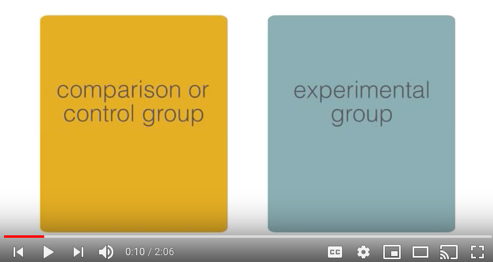
\includegraphics[width=0.5\textwidth]{figures/galileo/galileo-study-1}
  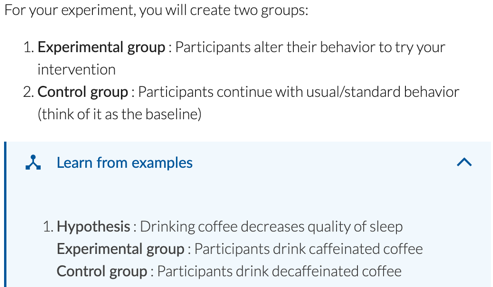
\includegraphics[width=0.5\textwidth]{figures/galileo/galileo-study-2}
  \caption[]
{Two conditions for experiment. In the Videos condition, participants accessed videos about experiment design. In the Galileo condition, participants accessed Galileo tool (which included the videos if participants wanted to see them). Both conditions provided the same content. \index{galileo-study-1}}
  \label{fig:galileo-study}
\end{figure}

\begin{comment}
%%%% TABLE 1 %%%%
\vspace{0.25in}
\begin{table}[!ht]
\caption[]{Demography info for 72 participants (all undergraduate students). Some participants did not complete portions of the survey.}

\vspace{-0.25in}
\begin{center}
\begin{tabular}{|p{1in}|p{2in}|p{3in}|}

\hline
Nationality: USA=37 &  \\

\hline
Hypothesis: 3 points & Is the cause/relation/effect specific?  \\

\hline
Measurement: 2 points & Are the cause and effect manipulated/measured correctly? \\

\hline
Conditions: 3 points  & Are the control and experi-mental conditions appropriate? 2pts \\
 & Do the conditions differ in manipulating the cause? 1pt \\

\hline
Steps: 2 points  & Are experimental steps clear for control/experimental conditions?  \\

\hline
Criteria: 2 points & Are the exclusion criteria correct and complete? Are the inclusion criteria correct? \\

\hline
Can the overall experiment be run as is? 1 point \\

\hline
\end{tabular}
\end{center}
\label{tab:rubric1}
\end{table}

Nationality	USA=37
No Answer = 6	China=11
Others = 18
Gender	Female = 47	Male = 24
Native English	Yes = 38	No = 34
Age	18-20=40
21-25 = 31	26-30=1

Ethnicity	Asian/Pacific=36
White = 11	Hispanic/Latino=14
Others = 11
Major	Biology=12
Cognitive Sci=12	Psychology=20
Others = 20
Used online learning 	Never=28
1 class=11	Occasional=16
2-5 classes=12


\end{comment}

\subsection{Participants}
\textit{Recruitment}: 72 participants were recruited from a Western US Research University (Table 2). 11 had no prior experience with experiment design; 61 had taken a course or equivalent. Expertise was counterbalanced across condi-tions.   

\subsection{Rubric for design-quality criteria for structure }

%%%% TABLE 2 %%%%
\vspace{0.25in}
\begin{table}[!ht]
\caption[]{Rubric for design-quality criteria for structure}

\vspace{-0.25in}
\begin{center}
\begin{tabular}{|p{1in}|p{2in}|p{3in}|}

\hline
Structure: 13 points &  \\

\hline
Hypothesis: 3 points & Is the cause/relation/effect specific?  \\

\hline
Measurement: 2 points & Are the cause and effect manipulated/measured correctly? \\

\hline
Conditions: 3 points  & Are the control and experi-mental conditions appropriate? 2pts \\
 & Do the conditions differ in manipulating the cause? 1pt \\

\hline
Steps: 2 points  & Are experimental steps clear for control/experimental conditions?  \\

\hline
Criteria: 2 points & Are the exclusion criteria correct and complete? Are the inclusion criteria correct? \\

\hline
Can the overall experiment be run as is? 1 point \\

\hline
\end{tabular}
\end{center}
\label{tab:rubric1}
\end{table}


\subsection{Measures}
The independent variable is access to Galileo/Videos. The study scored experiments via a 13-question rubric (Figure X), and recorded time taken. A blind-to-condition expert (a regular instructor of large, undergraduate courses on experiment design) provided the scores. Qualitative measures included how participants used the tool, where they faced challenges, and a post-experiment survey. A non-parametric Mann-Whitney test assessed the effect of condition on design quality. 

\subsection{Results}

\begin{figure}[h] 
  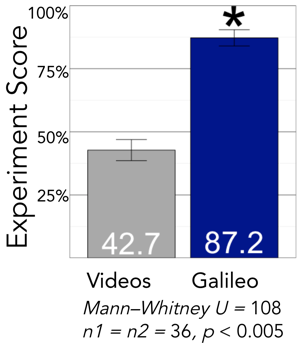
\includegraphics[width=0.5\textwidth]{figures/galileo/galileo-study1-7}
  \caption[]
{Access to Galileo improved the quality of experiment design. \index{galileo-study-1}}
  \label{fig:galileo-result}
\end{figure}

Galileo participants created higher-quality experiments (M = 11.3) than Videos participants (M = 5.6); Mann–Whitney U = 108, n1 = n2 = 36, p < 0.005 (Figure 7). Of the 36 designs rated in the top half, 29 were from Galileo condition. Galileo participants performed better on five out of six sections (all except hypothesis). There was no significant difference in the amount of time participants spent creating an experiment in the Videos (M = 30.8 mins) vs Galileo (M = 29.0 mins) conditions; Mann–Whitney U = 734, n1 = n2 = 36, p = 0.33 two-sided. 


\subsection{Study 1 Discussion}
As Galileo aims to improve tasks like experimental design, Study 1’s primary dependent variable was quality (as opposed to learning gains). Online video resources represent a common status quo: contemporary and bite-sized yet still static resources. This comparison enabled us to observe how Galileo’s procedural support changed design outcomes. Videos participants followed one of two strategies: 1) watch all the videos at once and then begin writing the experiment; or 2) begin designing the experiment and use the videos to fill in the gap when stuck. Like cramming, all-at-once watching floods the mind, perhaps making it difficult to use seen ideas [42]. By contrast, the search-when-needed approach interrupts people’s flow, replacing the attention on design with a task of locating needed information. Videos’ lower score and our observations, in conjunction with the literature, suggest contextually-integrated approaches like procedural support increase people’s useful adoption of information.   
Participants reported that the videos were slow and the interface provided sufficient examples. Participants in the Galileo condition opened and closed the videos in quick succession. Participants in the Videos condition, however, felt that the videos provided a refresher of some concepts they vaguely knew about. Did too much information (e.g. the inclusion of other concepts) in the Coursera course dilute performance? It’s possible; accessing the “right” moment in videos is a known research question [38]. 
Participants in both conditions expressed a lack of confi-dence in their chosen cause/effect measures. Some spent over 15 minutes searching for measures: one found a formal sleep-quality scale from Stanford researchers. Participants in both conditions mentioned that they enjoyed reflecting on their lifestyle/health ideas and thinking through how to transform an intuition into an experiment. Participants wished that Galileo was integrated with their class, describ-ing it as “hands on” and “DIY.” 

/subsubsection{Limitations}
This experiment found procedural support to yield higher-rated designs than watching videos. Important direction for future work will be to compare different approaches to procedural support, and exploring additional measures (e.g., novelty). 

\section{STUDY 2: DESIGN \& REVIEW EXPERIMENTS ONLINE}
The first study evaluated the efficacy of procedural support for designing experiments. The second study investigated the quality and nature of experiments; specifically, whether people a) create experiment designs that are structurally-sound, demonstrate insights from lived experiences, and have novel ideas, and b) provide useful feedback on experiment designs. 

\subsection{Method}
Participants used Galileo to design their experiments and review others’. Galileo’s landing page described why experiments are important and the importance of citizens’ contributions towards making discoveries. Upon logging in, participants could design an experiment (see Figure 2), review existing experiments (see Figure 3), or join an experiment (see Figure 4). 

\subsection{Recruitment}
Participants were recruited via online publicity. One recruitment focus was people curious about the microbiome because it is a domain where lived experience may inspire intuitions, and the science is nascent [52]. Galileo was promoted on the American Gut’s and their collaborators’ Facebook and Twitter pages. Galileo was added as a project on Open Humans (openhumans.org), posted on multiple subreddits pertaining to health and lifestyle, and introduced as an optional activity in assignments on the Gut Check Coursera MOOC [40]. Participation was voluntary and unpaid. 


%%%% TABLE 3 %%%%
\vspace{0.25in}
\begin{table}[!ht]
\caption[]{Rubric for design-quality criteria for Structure, Content, and Novelty}

\vspace{-0.25in}
\begin{center}
\begin{tabular}{|p{1in}|p{2in}|p{3in}|}

\hline
Structure: 13 points &  \textit{Described in Table 2} \\

\hline
Content  & \\
\hline
Personal? & Did the hypothesis draw from lived experience? \\
Popular? & Is the world already curious about this hypothesis (e.g. discussions on online fora)?  \\
Insightful? * Does the hypothesis link to existing science?  \\

\hline
Novel  &  \\
\hline
Is there a chance the world will learn something: absence of published research for this question? &  \\

\hline
\end{tabular}
\end{center}
\label{tab:rubric2}
\end{table}

\subsection{Measures}
Measures comprised structure, content, and novelty of experiment designs (Table 4) and usefulness of reviews. Raters with training in experiment design independently rated participants’ work, then discussed them to form a shared view of assessment. Next, each independently rated all experiments. The final score is the mean of their independent ratings. Moderate reliability was found between the two raters’ measurements [41]; m(ICC) = .62, 95% CI [.45, .75], (F(64,64)= 4.33, p<.001. 

Structure measures whether the design is correct and includes appropriate components. Content measures the subject matter of the idea driving the experiment design; it was rated as personal focus, popularity, and insightfulness of the hypothesis. Novelty was assessed as the potential to create new knowledge and operationalized as the lack of research papers about the specific hypothesis. Raters were instructed to assign points for a component (say hypothe-sis) if the experiment provided appropriate details about it. For example, the hypothesis “Text message reminder increases consumption of recovery snack” was rated to have a specific cause, a specific effect, and a clear relation between the two, while “Eating too much energy causes disturb [sic] sleep cycle” did not have a clear cause or effect. “Ingesting non-local food results in poor evacuation of fecal matter” was rated as novel because no published research addresses this (as per Google Scholar). Broad or vague hypotheses related to well-studied topics were not deemed novel (e.g. “Going to college increases grades”).

54 users from 16 countries created 66 complete experiment designs (Mdn=27 minutes). 37 users provided 205 descrip-tive review comments. Latest versions of complete experi-ment designs were scored as described above; incomplete experiments and older versions were removed from analy-sis. The anonymized data is at <URL>. 

\subsection{Study 2 Results}
\subsubsection{People Designed Structurally-Sound Experiments, and Drew from Personal Intuitions}
The mean score for the experiment was 10.3/13. On average, people scored higher than 75\% on 8 of 13 measures. 38\% of experiment designs came for people’s lived experiences; e.g., “eating yogurt makes a person have a more regular bowel movement”. Personal health and performance were big draws: 90\% of experiments sought to improve a health outcome. 
51\% of the experiments were rated as popular; their hypoth-eses were discussed on other online fora; e.g., “having dry mouth (or Sjogren's Syndrome) promotes the growth of less beneficial gut microbes”. Common themes included diet (dietary styles, alcohol, fermented foods), technology use (social media, laptop, mood) and alternative treatments (homeopathy), and health (sleep, pain, gut issues) (Figure 8). Apart from being structurally-sound, the best experi-ment designs shared two features: they shared a personal experience and linked to known research. For example, a user designed an experiment to test yogurt’s effect on bowel movement and shared their motivation: 

"For several months I have been producing Yogurt. This is fermented using commercial probiotics, Probiotic-10. My intuition was that since various microbe species were active in the making of the yogurt, this product can help relieve of the various digestive problems one persona can have. It happens that one of my sons was diagnosed with Ulcerative Colitis. among other things he was losing weight rapidly. After several weeks of consuming probiot-ics and/or the yogurt, he begun to recover."
17\% of hypotheses had novel insights that no published research addresses. For instance, “Avoiding foods high in lectins cures long-term post-infectious diarrhea” and “Drinking kombucha regularly reduces joint inflamma-tion/arthritis symptoms” are both hypotheses of interest to citizens and microbiome researchers alike.

\begin{figure}[h] 
\centering
  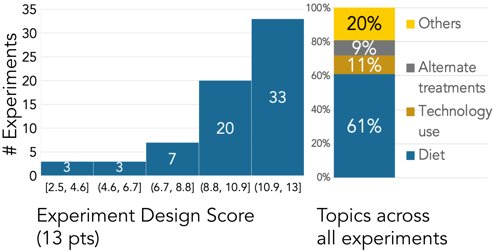
\includegraphics[width=1.0\textwidth]{figures/galileo/galileo-study2-1}
  \caption[]
{A) Most experiments were structurally-sound, scoring high on the structure rubric. B) Most experiments drew from personal experiences.. \index{galileo-study2-1}}
  \label{fig:galileo-result2}
\end{figure}

\begin{figure}[h] 
  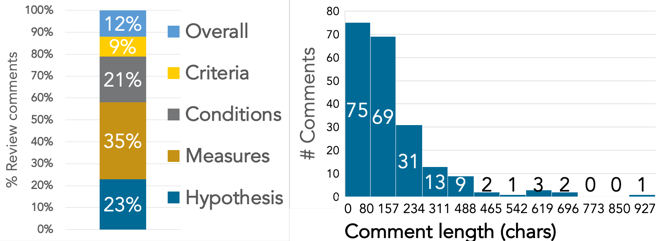
\includegraphics[width=0.66\textwidth]{figures/galileo/galileo-study2-2}
  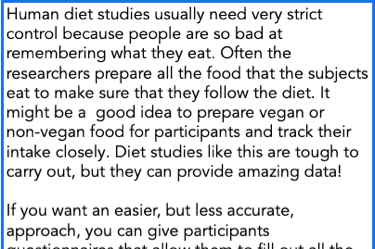
\includegraphics[width=0.33\textwidth]{figures/galileo/galileo-study2-3}
  \caption[]
{Summary of review A) Review comments were broadly distributed across all components of experimental design. B) Review comments ranged from 3 chars “yes” to 871 char long descriptions. C) The longest review comment described multiple problems with an experimental design while providing numerous actionable suggestions. \index{galileo-study2-2}}
  \label{fig:galileo-result2-2}
\end{figure}

\subsubsection{Reviewers Use Domain Knowledge to Improve Designs and Advocate for Participant Experience}
158 review comments (77\%) were rated useful; incorporat-ing them would improve the experiment. Average comment length was 140 characters ranging from 3 characters (“yes”) to 871 characters (Figure 9B,C). Most comments were direct responses to a rubric question hinting that the review interface helped people focus on the salient parts of an experiment design.
The most common comments sought improving structural correctness (38\%) by requesting specific details. For example, one reviewer questioned an experiment’s choice of Likert scale for mood saying, “A simplistic Likert scale seems like a bad idea. There has to be something better than this. At least a couple questions? Like, optimism, excitement, depression, anxiety?”. Reviewers provided the most comments (54\%) about the hypothesis and cause \& effect measures. People advocated for improving participant’s experience (18\%). Suggesting better data collection messages and times was a popular theme. We present two examples: 1) “People are not very good at remembering what they eat. Maybe an App like MyFitnessPal would be useful since it would allow participants to track all the food they eat without having to remember for too long.”, and 2) “How long do they [experiment participants] have to answer? What if they're eating dinner and can't get to it until 9pm?”.

14\% of comments demonstrated domain-specific knowledge E.g., one reviewer pointed out a conceptual mistake about a Type-1 diabetes experiment: “A1C is measured monthly and won't change after 1g. You mean the BG value?”. A1C refers to the average blood glucose value average levels over the past 3 months that is less susceptible to short term changes. BG here refers to the blood glucose value that depends on immediate glucose intake (among other factors). Surprisingly, reviewers barely drew from their personal experience when suggesting improvements (or at least, did not explicitly mention this was their personal experience). Some comments drew on counterfactual reasoning while thinking about how participants might “hack” an experi-ment. A comment on an experiment about social media use and steps walked asked, “…the timing of this [reporting steps taken] vs. social media use measure is off and that makes me worry about intervening use throwing things off (e.g. "phew! I've reported my facebook for the day, now I can go use it"?)”. 


\begin{figure}[h] 
\centering
  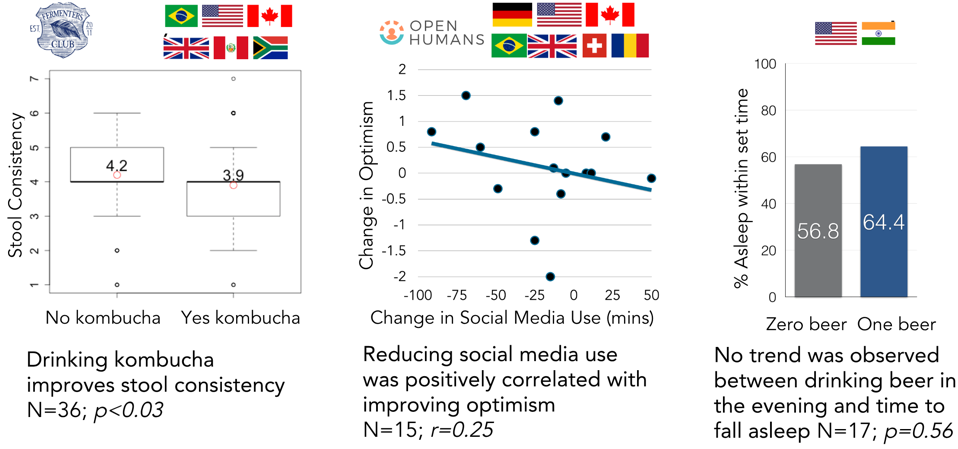
\includegraphics[width=1.0\textwidth]{figures/galileo/galileo-study3}
  \caption[]
{Three communities—Kombucha, Open Humans, Beer—designed and ran experiments; each ran for a week. The flags represent participants’ nationality. \index{galileo-study3}}
  \label{fig:galileo-result3}
\end{figure}

\begin{figure}[h] 
\centering
  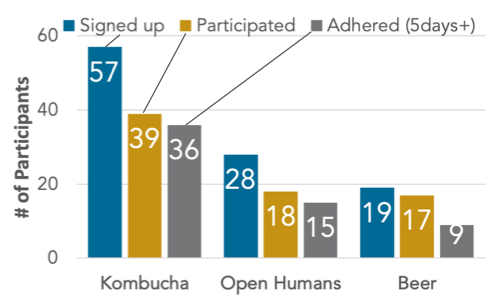
\includegraphics[width=0.5\textwidth]{figures/galileo/galileo-study3-1}
  \caption[]
{After signing up, a smaller fraction of people participated in Kombucha (68\%) and Open Humans (63\%) experiments than Beer (90\%). However, those who participated reported greater adherence in Kombucha (92\%) and Open Humans (83\%) compared to Open Humans (50\%). Reasons for non-adherence included being busy, annual leave, and brewers needing to check on the taste of Kombucha. \index{galileo-study3-1}}
  \label{fig:galileo-result3-1}
\end{figure}

\begin{figure}[h] 
\centering
  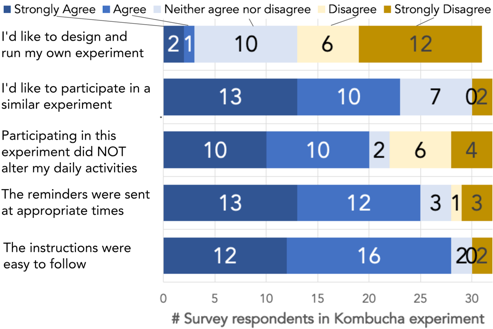
\includegraphics[width=0.5\textwidth]{figures/galileo/galileo-study3-2}
  \caption[]
{Participants in the kombucha experiment reported an overall positive experience expressing an interest to participant in another similar experiment (23/32). Most found the instructions easy to follow (28/32) and the reminders sent at appropriate times (25/32). \index{galileo-study3-2}}
  \label{fig:galileo-result3-2}
\end{figure}


\section{PEOPLE DESIGN, REVIEW, \& RUN EXPERIMENTS}
The previous two studies found that people generated novel, structurally-sound experiments. Might they success-fully run experiments with others? Participants from three communities — Kombucha, Open Humans, Beer —designed and ran experiments (Figure 10).  
Does drinking Kombucha improve stool consistency? Kombucha is a fermented tea drink popular in many parts of the world. Fermented foods (miso, yogurt, ayran, kefir) have been a staple in many cultures for thousands of years [13]. While there is widespread belief that kombucha “benefits the gut”, there is little published empirical evidence for these claims [24]. The experimenter hypothe-sized that kombucha supplies beneficial probiotics that help maintain normal stool consistency, and designed a between-subjects experiment.
Does reducing social media time increase optimism? Open Humans enables people to contribute personal data (e.g., genetic, social media, activity) for donation to research projects (openhumans.org). An experimenter investigated the relationship between social media and mood. Curious about the popular Facebook contagion study [17], an Open Humans member (openhumans.org) created a between-subjects experiment to investigate social media and optimism. 
Does drinking a beer in the evening help people fall asleep? Some people believe that a pint of beer in the evening helps them sleep by relaxing them; others think alcohol disturbs their sleep [57]. Alcohol helps people fall asleep but disrupts the REM cycle [22]. Still, it can be more convincing to see the evidence oneself. The experi-menter (a graduate student) tested the effect of beer on sleep time with a between-subjects experiment. 


\section{Results}
\subsection{Before the Experiment}
From initial design to launch — 37 (kombucha), 13 (Open Humans), and 11 (beer) days elapsed. Each experiment ran for a week.
Design and Review: None of the experimenters had previ-ously designed and run an experiment with people. All knew some concepts about experiment design; two have PhD degrees (in biology and ecology) and one is enrolled in a Computer Science PhD program. The experimenters are Brazilian, German, and US nationals. While the three experimenters had lived experience of their experiment’s topic, they had never scientifically studied it.
Reviewers provided a total of 104 boolean answers and 32 detailed comments. Comments focused on two themes. First, reviewers helped make the hypothesis and measures more specific; e.g., an experimenter started with the question “Does drinking a beer in the evening help you get to bed on time?”; the reviewers nudged the experimenter to creating the more specific hypothesis: “Drinking a 5% ABV (0.5%) beer between 6PM and 8PM local time helps people fall asleep no more than 30 minutes past their desired bed time.” A reviewer criticized Kombucha experi-ment’s 5-point Likert scale for bloatedness as overly vague. In response, the experimenter found and adopted the Bristol stool chart—a picture-based scale that is the industry standard [66]. Second, reviewers suggested improving data quality by instructing participants to skip confounding activities. For example, reviewers pointed out that caffeine and alcohol interact. The experimenter addressed this in instructions asking participants to abstain from coffee and alcohol. All issues that reviewers raised were tightly connected to Galileo’s review rubric (Figure 3). At the end of review, the three experiment designs used appropriate measures, provided a minimal-pairs design, tracked con-founds, and provided appropriate criteria for participation.
Pilots: Three lessons emerged. First, some participants were loath to look at their stool. Since viewing one’s stool is necessary, the experimenter added an inclusion criterion enforcing this. Second, some participants reported eating other fermented foods in the process; the experimenter modified the instructions for participants to not consume these. Third, after failing to recruit sufficient participants, the experimenter collaborated with a kombucha fermenter in an American city who knew more kombucha enthusiasts. Before testing for the effect of social media, an Open Humans member piloted a study on the effect of 30 extra minutes of aerobic exercises on sleep. However, potential participants were loath to alter their lifestyle this dramati-cally, and so the experimenter abandoned the study. 
Finding participants: The Kombucha experimenter publi-cized the experiment on Instagram, Twitter, and newsletter; they also created a poster, and reached out to enthusiasts in their city in Brazil and an American city. The Open Humans experimenter recruited on social media, a mailing list, and the Open Humans Slack channel. The beer experi-menter reached out to peers interested in community experimentation and/or the effects of alcohol. At least one potential participant in each of the three experiments was excluded because of inclusion/exclusion criteria. 

\subsection{During the Experiment}
Retention: 57 people signed up for the kombucha experi-ment; 36 completed it (68\%). Retention rates were similar for the Open Humans experiment (63\%) and higher for beer (90\%) (Figure 11). 78\% of dropouts occurred in the first 48 hours. The reasons participants reported for dropping out included lack of interest, holidays, and work travel.
Adherence: Kombucha garnered 76\% adherence: 86\% for days of no kombucha, and 70\% when asked to drink kombucha. Most Open Humans participants reported high adherence, cutting social media use in half or more (Figure 11). Each day, an average of 54\% of participants in the beer experiment reported following the condition requirement (drinking 1 or 0 beers by 8PM). 15 of 17 failed to comply on at least one day.
Some participants disclosed confounds and reasons for non-adherence. For example, drinking alcohol was a reported confound, because it might affect kombucha’s impact on the body. Similarly, participants’ non-adherence reports included scheduled disruptions like travel and holidays and work responsibilities like brewers needing to check on the taste of kombucha. Non-adherence for the beer experiment included drinking wine rather than beer, drinking after 8PM, drinking more than one beer, or not drinking in the drink-one condition.

Data Collection: Most American participants selected text solicitations (86\%); participants elsewhere received email solicitations due to varying regulations around automated text messages (e.g., replying to an automated text message in Brazil or India is infeasible since the source number is masked). 56% of participant responses came within 30 minutes of the solicitation; 21% of responses took more than 90 mins. Participants sparingly responded to follow-up questions. Experimenters used the remind participant button 2 (kombucha) and 3 (Open Humans) times to remind participants with missing data.
Clarifying questions: The experiment requested that all participants adhere to the protocol as much as possible without harming their health. Participants could ask the experimenter (via the platform) if confused. Participants’ clarifying questions focused on measurements (e.g., measuring stool consistency once during the day or multi-ple times) and specific lifestyle choices (e.g., consuming probiotics while drinking kombucha?). Participants in kombucha experiment reported an overall positive experi-ence (Figure 12).

\subsection{Study 3 Discussion}
Our results point at three challenges in democratizing experimentation: 1) the three experimenters had advanced degrees, 2) two of the three completed experiments were underpowered, and 3) experiment participants demonstrated varying levels of adherence. 
Do successful citizen-led experiments require prior exper-tise? While an advanced degree is not a pre-requisite, having one confers an advantage. This is unsurprising; contributions to open access web platforms are rarely uniform across educational levels. MOOCs are dispropor-tionately completed by learners from more-affluent and better-educated neighborhoods [29], and 73\% of citizen scientists and Wikipedia contributors have advanced degrees [1,65]. 
Why were all three experiments run by people with ad-vanced degrees? One reason could be self-selection: those without prior expertise in experimentation might have opted out of running an experiment. This is weakly supported by data: all 36 participants in the kombucha experiment enjoyed the experiment and wanted to partici-pate in more experiments (Figure 14). However, only two participants wanted to design and run follow-up experi-ments; both have an advanced degree. While simply asking people to contribute might work for traditional citizen science projects, experimentation might be a bigger leap. We suggest two improvements. First, reduce effort by providing ready to run experiments; common health and lifestyle topics such as coffee consumption and sleep might be good candidates. Running a sample experiment enables people to pilot the platform before testing their ideas while also potentially making them comfortable with the idea of experimentation itself. Second, support a growth mindset [21]: e.g. the platform can emphasize that anyone can learn how to run an experiment.
Another reason for experimentation by those with advanced degrees could be their awareness of potential participants. All three experimenters had access to people who were interested in similar topics; e.g., the Open Humans experi-menter received both participants and feedback for their idea from the group’s slack community. Such affinity spaces are known to provide potential participants as well as social support [26]. To tackle this, the design workflow can nudge the creator to start their experiment design by thinking of topics relevant to their social connections.

\subsubsection{Guidance Techniques to Enable Citizens to Recruit Others}
Two of the three completed experiments were underpow-ered. Citizen experimenters learned what many scientists know: recruiting participants is time-consuming. This suggests that a good experimental design is not enough and recruiting is the next challenge for citizen scientists on their way to develop meaningful knowledge. While the absence of shared knowledge with experts can sometimes give novices’ work a boost (e.g. identifying green pea galaxies on Galaxy zoo), it’s less useful when the lack of knowledge is a hindrance. Tools for training and collaboration can help by clearly conveying the importance of getting enough participants; enabling experimenters estimate what “enough” is; and providing sources and strategies to recruit participants.
Citizen experimenters aren’t as ardent about sufficient participation numbers as professional scientists. One important piece of technical knowledge is performing power analysis before running the experiment. Additionally, following the lead of data journalists [28], conveying results through real-world effect sizes—such as additional years you’ll live—might be useful. Moreover, the experi-menter need not find all the participants by themselves. Akin to a Clinical Research Coordinator, a separate re-cruitment role can help the experimenter rope in others to help out. Participants signed up for an experiment can also assist by suggesting others ala snowball sampling.
How might we help increase participation? Common reasons why people join expert-led experiments include [55]: to help find an answer to a question that personally affects them, to gain access to potential treatments, and for credit or monetary compensation. Moreover, the trust placed in institutional researchers might not extend to citizen experimenters [14]. 
Adherence, however, remains a challenge. The opportunity to contribute to science is exciting (e.g. kombucha experi-ment participants mentioned this as a motivation). While altering one’s lifestyle for a day might not be very difficult for many people, doing the same for a week (or more) might be tedious enough to entirely avoid participating, drop out after signing up, or not adhere to the instructions.
Drawing on findings from social computing and crowd-funding [34,37], we suggest four remedies to improve both participation and adherence numbers: 1) increase participant trust by sharing more information about the experiment’s goals, approximate effort expected, and the experimenter’s biography; 2) implement activation thresholds to make social reciprocity explicit for group activities and to reduce potentially wasted efforts [12]; 3) leverage participation from communities with already strong ties and common goals; 4) allow people to pre-register for topics of interest so they might join relevant experiments created at a later date [4].
Our study did not provide experimenters or participants monetary compensation. Consequently, people’s motiva-tion is more intrinsic, which has benefits [54] (e.g. telling people the importance of their work improves performance [9]), but also empirically shows a high dropout rate. Compensation may help some citizen science experiments. 

\section{DESIGN IMPLICATIONS FOR KNOWLEDGE WORK}
We suggest three heuristics for systems that chunk complex knowledge work: separate roles, provide interactive guid-ance, and facilitate iteration. These ideas extend minimal-ism to design learning experiences [53]. 
1 Identify roles. People, especially novices, often struggle to get started. Role-based approaches confer three benefits: clean delineation of responsibilities improves chances of task completion, clustering similar tasks reduces overhead and increases consistency; and people can decide their contribution levels. Procedural support operationalizes minimalism by co-locating tailored learning resources with specific steps.
2 Provide procedural support for just-in-time domain-expertise. A diverse audience might not interpret instruc-tions consistently, or fail to translate textbook definitions to practice. Our results show that people are good at interpreting procedural support (like examples) for their use case. Creating such learning resources using the crowd or even learners themselves could reduce the effort needed [38]. 
Checklists, cognitive aids, and tutoring systems exploit chunking as a means of onboarding new participants in a community of practice. For checklists, these chunks are usually static and expert-designed. A powerful benefit of interactivity is the opportunity for personalization. To reduce the time spent designing scaffolds and workflows, reuse lessons from other tools. 
 	Our first two heuristics focus on the authoring piece. Our third heuristic focuses on the reviewing piece. In contrast with cognitive aids and tutoring systems that “bake in” knowledge, our review step—like learnersourcing [38]—leverages the crowd for customized feedback. Structured reviewing—like Galileo—simultaneously discourages the lazy shortcut of superficial reviewing, and lowers the cognitive burden of providing deep, actionable feedback. 
3 Handle errors using iterations. Most first drafts have errors. Feedback can be provided by experts [20,60], peers [6,44], software [19], or even oneself [6,60]. Support iterations and pre-task training can counter concerns of superficial reviews. Why? Scaffolded questions and checklists help people reflect on their work at every step, especially when the system fails to automatically tackle inconsistencies for open-ended work.

\section{Conclusion}
This paper investigated citizen-led experimentation with novel procedural support. Three empirical investigations tested this approach. For us, the most striking result is that online volunteers collaboratively performed scientific experimentation without any expert help by drawing on their lived experience. Our work also illustrates the chal-lenge of helping novices successfully execute a complex knowledge task. Specifically, finding and retaining partici-pants and making the platform accessible to a broader audience emerged as key challenges. With systems that enable citizen-led experimentation, people can potentially match scientists’ knowledge with their lived experiences to create insights both for themselves and for the scientific community. More generally, we hope that our work suggests ways to build systems that provide just-in-time domain expertise for knowledge work. Such systems can enable novice-led work that is personally meaningful, and situated in people’s lived experiences.

\section{Do Citizen  Experiments Benefit or Harm Society?}
One challenge of modern life is the increasing layers of social and technical infrastructure that separate the creation of knowledge from its everyday use. This divorce makes it difficult to wisely assess and use knowledge. This paper has outlined the positive potential for citizen designed experiments, a greater range of perspectives, participation, and understanding. It’s worth considering the risks. The primary concern we have is that a poorly designed experiment with a faulty conclusion influences people in fraught ways. 
At its best, over time scientific experiments expand human knowledge and correct mistakes when they occur. However, sometimes the popular press reports a headline-grabbing result that is inaccurate, but not the subsequent correction and elaboration. Particularly with science, when ideas are newsworthy but low-quality, people can incorporate misguided ideas in a way that be difficult to dislodge. Perhaps the most notorious example is the (debunked) claim that vaccines, especially MMR vaccine, cause autism by disrupting the body’s microbial composition  and/or introducing harmful chemicals. At a time of rising autism diagnoses, this claim terrified parents and continues to impede childhood vaccination more than two decades later . Furthermore, the 20th century offers many examples of pervasively-adopted chemicals (such as lead in paint and gasoline, and asbestos in buildings) that were later found to be toxic. Wakefield’s publication linking MMR vaccine to autism (later retracted) was a serial case study [24], not an experiment. While sharing case studies can help identify valuable leads for further study, the small size and biased selection create enormous risk of confounds and spurious relationships. (In this case, unidentified correlated timing in the measures and undisclosed financial ties by the author further clouded the picture.) Currently, most readers cannot fully grasp the evidentiary difference between a small case study and a rigorous controlled experiment. Our hope is that democratizing the doing of science may help the public interpret science news and reduce the risk of leaping to conclusions.
Because not all experiments are appropriate for people to run, some gatekeeping of citizen experiments might be necessary. 62 of 66 complete designs were posted online on Galileo for others to view; the primary author took 4 down because the research team identified them as risky. For example, one removed design sought to investigate the effect of colloidal silver on cognitive performance. There is a community that believes colloidal silver (tiny particles suspended in liquid) to have beneficial properties [47]. While the designer may be well-intentioned, consuming colloidal silver can cause irreversible damage such as skin discoloration, and the NIH has sued manufacturers for misleading claims [29]. Galileo offers keyword triggers for alerting both the designer and the research team of possibly dangerous experiments. For example, an experiment containing “cancer” or “CBD” triggers an email to the research team; use of the word “cancer” indicates potential health risks for participants (who might be cancer patients) while “CBD” indicates potential legal risks across many places around the world.
can people actually find answers to questions suggested by experts who are too busy to run that experiment themselves -- complementing clinicians 1. see work around patient-led experimentation
Sifting through ideas expressed by people for experimentation, we believe citizen experiments seem well suited for ideas that meet three criteria; they must 1) be scientifically tenable, 2) combine high excitement with low efforts, and 3) provide zero to no risk. S cientifically tenable means that the experiment answers a gap in research literature, minimizes placebo effects, and yields results in a week with a high likelihood. To be low-effort, all the experimental steps (including reporting data) should be easy to understand and perform. Finally, the experiment should not provide any cause of harm to participants and it should be legally and ethically permissible across countries and cultures. As a crude beginning, this can be operationalized as the existence of numerous anecdotes about potential upsides with none or well understood downsides. For instance, bee venom reduces Lyme disease symptoms (an idea proposed on the platform) is an idea with anecdotal benefits but the existence of venom implies non-trivial possibility of self-harm.

